\documentclass[a4paper,conference]{IEEEtran}

\usepackage{cite}
\usepackage{amsmath,amssymb,amsfonts}
\usepackage{graphicx}
\usepackage{booktabs}
\usepackage{url}
\usepackage{enumitem}
\usepackage{tikz}
\usetikzlibrary{arrows.meta,positioning}

\setlist{itemsep=0pt,parsep=0pt,topsep=2pt,leftmargin=*}
\setlength{\textfloatsep}{7pt plus 1pt minus 2pt}
\setlength{\floatsep}{6pt plus 1pt minus 2pt}
\setlength{\intextsep}{7pt plus 1pt minus 2pt}
\setlength{\dbltextfloatsep}{7pt plus 1pt minus 2pt}

\begin{document}

\title{A Configurable Dynamic-Fee Hook Framework for Uniswap v4 Liquidity Pools}

% Confirm full names, affiliations, and e-mail addresses before submission.
% \author{\IEEEauthorblockN{Yash Madhwal, Ivan Frolov, Vasiliy Grachev, Anton Ledrov and Yury A. Yanovich}
% Anton  Ledrov  ledrov.aiu@phystech.edu  Russia  Moscow Institute of Physics and Technology, Moscow, Russia
% \IEEEauthorblockA{Faculty of Computer Science, HSE University\\
% Moscow, Russia}}

\maketitle

\begin{abstract}
  Automated market makers typically apply a static swap fee although volatility, order flow, and liquidity-provider exposure vary over time. Uniswap v4 makes fee logic programmable through hooks, but implementing and comparing alternative policies still requires protocol-specific contracts, deployment scripts, data feeds, simulations, and analysis tools. This paper presents a configurable framework that unifies these components. It provides a shared Solidity abstraction and templates for block-adaptive, deal-adaptive, asymmetric, MEV-related, and peg-stability fee policies; optional Chainlink-compatible price access; reusable Foundry/Anvil deployment and testing utilities; and a web configurator that exposes parameters and generated source code. The same interface exports a deployable project and runs historical-data replay using Binance observations. A prototype execution over an ETH/SHIB trace processes 1,492 simulated swaps and produces external-price, price-ratio, pool-price, volume, fee, and liquidity-provider metrics. The evidence establishes end-to-end implementation feasibility, not economic superiority over static fees. The framework contributes reproducible engineering infrastructure through which dynamic-fee policies can be inspected, deployed, and evaluated under a common workflow.
\end{abstract}

\begin{IEEEkeywords}
  automated market makers, decentralized exchanges, dynamic fees, Uniswap v4, smart-contract hooks, liquidity provision
\end{IEEEkeywords}

\section{Introduction}
\label{sec:introduction}

Decentralized finance (DeFi) implements exchange, lending, derivatives, and asset-management services through publicly executable smart contracts~\cite{werner2022sok}. Within this ecosystem, decentralized exchanges (DEXs) remove the need for a custodial order-matching intermediary. Many DEXs use constant-function automated market makers (AMMs), which accept trades against reserves according to a deterministic function~\cite{angeris2019analysis,angeris2022multiasset}. Uniswap popularized the constant-product design and subsequently introduced concentrated liquidity, allowing liquidity providers (LPs) to allocate capital within selected price ranges~\cite{adams2020uniswap,adams2021uniswapv3}. These mechanisms enable permissionless market creation and continuous on-chain execution, but they also transfer inventory and adverse-selection risk to LPs. Although the term \textit{dynamic pricing} is sometimes used broadly in this context, it is critical to clarify that this framework controls the trading fee parameter, not the asset price itself. In AMM systems, the price is determined by the pool invariant and liquidity state; this framework solely manages the adaptive rules for fee extraction to balance LP protection and trader execution costs.

An AMM price changes only when a transaction updates the pool state. When an external market moves first, arbitrageurs trade against the stale pool until the price discrepancy is no longer profitable. The resulting rebalancing changes the composition and value of the LP position. Impermanent loss compares that position with holding the deposited assets, whereas loss-versus-rebalancing (LVR) isolates the cost of being passively rebalanced at stale prices relative to a continuously rebalanced benchmark~\cite{milionis2022lvr}. Concentrated liquidity adds a further allocation trade-off: narrow ranges increase fee share while active, but cease earning fees after the market exits the range and can require costly repositioning~\cite{fan2021strategic}.

Swap fees are the primary compensation LPs receive for bearing these risks, directly impacting the magnitude of impermanent loss~\cite{Vlasov2025Impact}. A static fee, however, must serve incompatible market states. During stable periods, a high fee worsens execution and can redirect order flow to competing venues. During volatile periods, a low fee may not compensate LPs for informed or arbitrage flow. The appropriate fee therefore depends on variables such as volatility, external-price displacement, pool depth, trade direction, and the amount of uninformed volume. Dynamic mechanisms attempt to price this changing exposure instead of selecting one fee ex ante.

Recent research formalizes this trade-off from several directions. Fritsch~\cite{Fritsch_2021} analyzes optimal fee structures for constant function market makers, while Lebedeva \emph{et al.} evaluate block-adaptive, deal-adaptive, and oracle-informed asymmetric fees~\cite{lebedeva2025dynamic}. Baggiani \emph{et al.} derive dynamic policies through stochastic control~\cite{baggiani2025optimal}, while Campbell \emph{et al.} study optimal fees when an AMM competes with a centralized exchange~\cite{campbell2025optimal}. Agent-based work further incorporates latency, heterogeneous traders, arbitrageurs, and maximal-extractable-value (MEV) searchers~\cite{dinosse2026dynamic}. Collectively, these results motivate adaptive fees, but their economic models do not remove the engineering burden of implementing multiple policies consistently on a production-oriented AMM.

Uniswap v4 provides the missing protocol primitive. Its hooks are external contracts invoked at selected points of a pool's lifecycle; a dynamic-fee pool can update its stored LP fee or obtain a per-swap override from a hook~\cite{adams2024uniswapv4,uniswapDynamicFees}. Yet a usable experiment requires more than the fee equation. Developers must declare and encode callback permissions, deploy core and periphery contracts, create a compatible hook address, initialize a pool, provide test assets and price feeds, replay trading activity, and calculate comparable outputs. Implementing these tasks separately for every policy undermines reproducibility and makes differences in surrounding infrastructure difficult to distinguish from differences in fee logic.

This paper addresses that systems gap with a configurable development and evaluation framework for Uniswap v4 dynamic-fee hooks. It connects a common Solidity contract structure, local protocol deployment, historical-data replay, metric extraction, visualization, and project generation. The framework deliberately exposes the generated source: it assists development rather than replacing code review with an opaque configurator.

The contributions are:
\begin{itemize}
  \item A modular contract and deployment architecture that separates fee-policy logic from Uniswap v4 lifecycle and bootstrap code.
  \item Configurable templates spanning block- and trade-adaptive behaviors, specifically implementing Exponential Moving Average (EMA) and Welford’s online algorithm for variance-based fee calculation, alongside MEV-oriented and peg-stability policies.
  \item An integrated Foundry/Anvil experiment workflow that replays historical observations and collects pool-level outputs.
  \item A browser interface that presents policy parameters and source, exports a self-contained project, and visualizes simulation results.
\end{itemize}

The current artifact is evaluated as an engineering prototype. The available trace demonstrates that the full workflow executes, but lacks the fixed-fee baselines and repeated trials required to claim improved LP performance. This boundary is maintained throughout the paper.

\section{Background and Related Work}
\label{sec:background}

\subsection{AMM Fees and LP Exposure}

For reserves $x$ and $y$, a constant-product AMM maintains
\begin{equation}
  xy=k,
  \label{eq:constant-product}
\end{equation}
apart from fees, rounding, and protocol accounting. If a trader supplies $\Delta x$ and the proportional fee is $f$, the simplified output is
\begin{equation}
  \Delta y=y-\frac{xy}{x+(1-f)\Delta x}.
  \label{eq:swap-output}
\end{equation}
Thus $f$ affects both LP revenue and trader execution. Formal analyses show how constant-function markets track reference prices through arbitrage and generalize beyond two-asset products~\cite{angeris2019analysis,angeris2020improved,angeris2022multiasset}.

Let $V_{\mathrm{LP}}(T)$ be the terminal marked-to-market LP position, $V_{\mathrm{H}}(T)$ the value of holding the original assets, and $R_f(T)$ fee income in the same numeraire. A value-based loss and its fee-adjusted form are
\begin{align}
  IL(T)&=V_{\mathrm{H}}(T)-V_{\mathrm{LP}}(T),\label{eq:il}\\
  L_{\mathrm{net}}(T)&=IL(T)-R_f(T).\label{eq:netloss}
\end{align}
This accounting distinction matters: an adaptive fee may compensate LPs through revenue without eliminating the stale-price mechanism that produces adverse selection. LVR makes that mechanism explicit by comparing the AMM with continuous rebalancing at the reference price~\cite{milionis2022lvr}, and recent work has further quantified the specific profitability zones where fee accumulation can turn impermanent loss into a sustainable gain~\cite{melnikov2026impermanent_gain}.

A static pool sets $f_t=f$. A dynamic policy instead evaluates
\begin{equation}
  f_t=\mathcal{F}(s_t,z_t;\theta),
  \label{eq:policy}
\end{equation}
where $s_t$ is observable on-chain state, $z_t$ optional external information, and $\theta$ a parameter vector. Directional policies return $f_t^{0\rightarrow1}$ and $f_t^{1\rightarrow0}$ separately, for example charging more when a swap moves the pool farther from an external reference.

\subsection{Dynamic-Fee Research}

Dynamic policies use different proxies for adverse conditions. Volatility-based mechanisms react to price variability; inventory policies account for reserve composition; oracle-informed policies use pool-to-reference deviation; and flow-based rules use recent volume, trade size, or direction. Lebedeva \emph{et al.} compare block-level, transaction-level, and idealized oracle-informed mechanisms and find improved LP outcomes under their simulation assumptions~\cite{lebedeva2025dynamic}. Baggiani \emph{et al.} identify two regimes in which fees balance arbitrage deterrence against attracting noise traders~\cite{baggiani2025optimal}. Campbell \emph{et al.} similarly show that volatility and competing-venue costs jointly determine fee choice~\cite{campbell2025optimal}. Recent agent-based analysis suggests that dynamic schedules may improve hedged LP profitability mainly by increasing compensation in toxic states, rather than mechanically eliminating LVR~\cite{dinosse2026dynamic}.

These works optimize or compare economic policies. Our contribution is complementary: a common implementation substrate for configuring, deploying, and replaying multiple fee rules as Uniswap v4 hooks. It enables a later controlled economic comparison while keeping the surrounding software path fixed.

The closest studies therefore occupy distinct levels. Formal CFMM work supplies the market foundation~\cite{angeris2019analysis,angeris2022multiasset}; LVR supplies an LP-risk benchmark~\cite{milionis2022lvr}; and dynamic-fee studies supply candidate policies and economic hypotheses~\cite{lebedeva2025dynamic,baggiani2025optimal,dinosse2026dynamic}. This paper operates at the systems level by making several rules deployable and observable through one protocol-specific path. Neither level replaces the other: a framework without controlled baselines cannot demonstrate economic benefit, while a fee model without reproducible implementation leaves integration effects unmeasured.

While protocols like Balancer V3, Curve V2, and Algebra Finance have introduced internal mechanisms for adaptive fees or volatility-based adjustments, these features are tightly coupled to their specific protocol architectures. They do not provide a unified, external management layer. Consequently, researchers and developers cannot easily deploy, configure, monitor, and compare multiple fee strategies across a standardized infrastructure. This framework fills that gap by providing a protocol-agnostic (within the Uniswap v4 ecosystem) external contour for strategy lifecycle management.

Table~\ref{tab:relatedwork} condenses this distinction. Prior studies primarily contribute market models, LP-risk measures, or fee policies. The present work does not replace those results; it supplies the implementation and replay path needed to instantiate and compare policy families on Uniswap v4.

\begin{table*}[t]
  \caption{Positioning relative to representative AMM and dynamic-fee research.}
  \label{tab:relatedwork}
  \centering
  \footnotesize
  \begin{tabular}{p{3.7cm}p{5.8cm}p{5.7cm}}
    \toprule
    \textbf{Work} & \textbf{Primary contribution} & \textbf{Relationship to this framework}\\
    \midrule
    Angeris \emph{et al.}~\cite{angeris2019analysis,angeris2022multiasset} & Formal analysis and optimization of constant-function markets & Supplies the AMM foundation, not hook tooling\\
    Milionis \emph{et al.}~\cite{milionis2022lvr} & LVR formulation for adverse-selection cost & Supplies an LP-risk benchmark for future evaluation\\
    Lebedeva \emph{et al.}~\cite{lebedeva2025dynamic} & Block-, deal-, and oracle-informed fee policies & Supplies a policy family represented by the templates\\
    Baggiani \emph{et al.}~\cite{baggiani2025optimal} & Stochastic-control formulation of dynamic fees & Supplies theoretical fee-design guidance\\
    This work & Configurable contracts, deployment, replay, project export, and visualization & Supplies shared Uniswap v4 experimentation infrastructure\\
    \bottomrule
  \end{tabular}
\end{table*}

\subsection{Uniswap v4 and External Data}

Uniswap v4 stores pools in a singleton \texttt{PoolManager} and settles intermediate balance changes through flash accounting~\cite{adams2024uniswapv4}. Hooks attach custom logic to initialization, liquidity, swap, and donation callbacks. Their enabled permissions are encoded in low-order address bits, so deployment must produce an address matching the declared callbacks~\cite{uniswapHooksDocs,uniswapHookDeployment}. For dynamic pools, a hook can call \texttt{updateDynamicLPFee} or return a per-swap override from \texttt{beforeSwap}~\cite{uniswapDynamicFees}. OpenZeppelin provides reusable bases for callback validation and fee management, including \texttt{BaseDynamicFee} and \texttt{BaseOverrideFee}~\cite{openzeppelinHooks}.

Oracle-informed policies require a reference unavailable from the pool itself. Chainlink Data Feeds expose aggregated observations to contracts~\cite{chainlinkFeeds}. For two USD-denominated feeds, the external ratio is $r_t^{\mathrm{ext}}=p_{0,t}/p_{1,t}$. Production logic must normalize decimals and reject invalid or stale rounds. In the framework, deterministic mocks reproduce historical observations; they validate integration logic, not the timing or fault behavior of a live oracle.

\section{Framework Design}
\label{sec:framework}

\subsection{Layered Architecture}

The framework has four layers. The \emph{contract layer} contains hooks, base contracts, and interfaces; it computes directional fees, maintains policy state, validates callbacks, and interacts with \texttt{PoolManager}. The \emph{deployment layer} uses \texttt{BaseScript}, \texttt{Deployers}, and \texttt{HookHelpers} to create mock tokens and feeds, deploy Uniswap artifacts and the selected hook, and initialize its pool. The \emph{experiment layer} combines Forge tests, \texttt{Simulation.t.sol}, data utilities, and the result parser to replay observations and record price, volume, fees, holdings, and LP metrics. Finally, the \emph{application layer} uses Flask and browser code to select and configure hooks, display source, export projects, run simulations, and present results. Foundry supplies Solidity-native compilation, tests, and scripts, while Anvil provides the local EVM~\cite{foundryBook,anvilBook}; Flask implements the local HTTP interface~\cite{flaskDocs}.

The workflow is: (1) select a hook; (2) load its annotated description, parameters, and Solidity template; (3) set parameter values; (4) generate a configured copy; (5) export the project or choose a historical trace; (6) deploy the local infrastructure; (7) execute swaps; and (8) parse and visualize results. Policy code is therefore varied without rebuilding every supporting component.

The separation also defines explicit data boundaries. Configuration data flows from the browser to the generator; Solidity artifacts flow from the generator to the compiler and exporter; historical observations flow from the acquisition utility to the simulation; and emitted values flow from Forge to the parser and plots. The canonical hook sources are never simulation results, and the raw market observations are not inferred from the pool. This distinction prevents a configured constant, a reference-market input, and an endogenous pool output from being treated as interchangeable evidence.

Figure~\ref{fig:workflow} makes the execution boundary explicit. A user choice and an annotated hook template enter the configurator, which produces a concrete Foundry project. The deployment scripts then instantiate the selected contract together with the local Uniswap dependencies. Historical observations enter only at the replay stage, where mock feeds and swap inputs drive contract execution. Finally, emitted values are parsed into metrics and figures. The generated project can also leave the workflow directly for independent inspection and execution; using the web interface is not required after export.

\begin{figure*}[t]
  \centering
  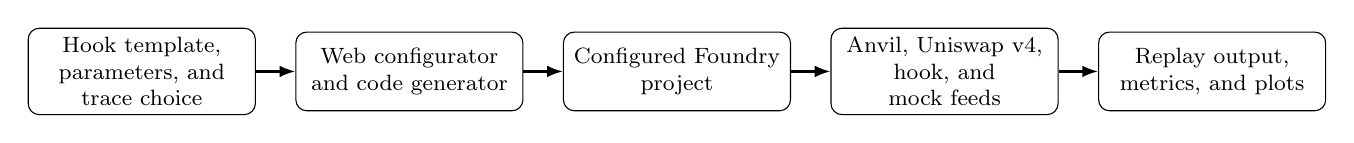
\begin{tikzpicture}[
      node distance=5mm,
      box/.style={draw, rounded corners, align=center, minimum height=10mm,
      text width=2.65cm, font=\footnotesize},
      flow/.style={-{Latex[length=2mm]}, thick}
    ]
    \node[box] (input) {Hook template,\\parameters, and trace choice};
    \node[box, right=of input] (config) {Web configurator\\and code generator};
    \node[box, right=of config] (project) {Configured Foundry\\project};
    \node[box, right=of project] (chain) {Anvil, Uniswap v4,\\hook, and mock feeds};
    \node[box, right=of chain] (result) {Replay output,\\metrics, and plots};
    \draw[flow] (input) -- (config);
    \draw[flow] (config) -- (project);
    \draw[flow] (project) -- (chain);
    \draw[flow] (chain) -- (result);
  \end{tikzpicture}
  \caption{End-to-end configuration, deployment, and replay workflow.}
  \label{fig:workflow}
\end{figure*}

Two properties follow from this organization. First, policy comparison can reuse the same contract graph and replay machinery, reducing infrastructure variation between experiments. Second, every transition produces an inspectable artifact: configured Solidity, deployment logs, Forge output, or generated plots. This improves debuggability and makes it possible to identify whether a failure originates in generation, deployment, contract execution, data preparation, or result parsing.

\subsection{Configuration and Generation}

Figure~\ref{fig:configurator} shows the configurator. For template $C$ and parameters $\theta=[\theta_1,\ldots,\theta_n]$, generation produces
\begin{equation}
  C_{\theta}=\mathcal{G}(C,\theta).
  \label{eq:generation}
\end{equation}
The current implementation substitutes exposed values into a generated copy and leaves the canonical template unchanged. The interface restricts hook selection to known templates, but textual substitution is not a typed Solidity transformation; this limitation motivates the typed schema discussed in Sec.~\ref{sec:discussion}.

\begin{figure}[t]
  \centering
  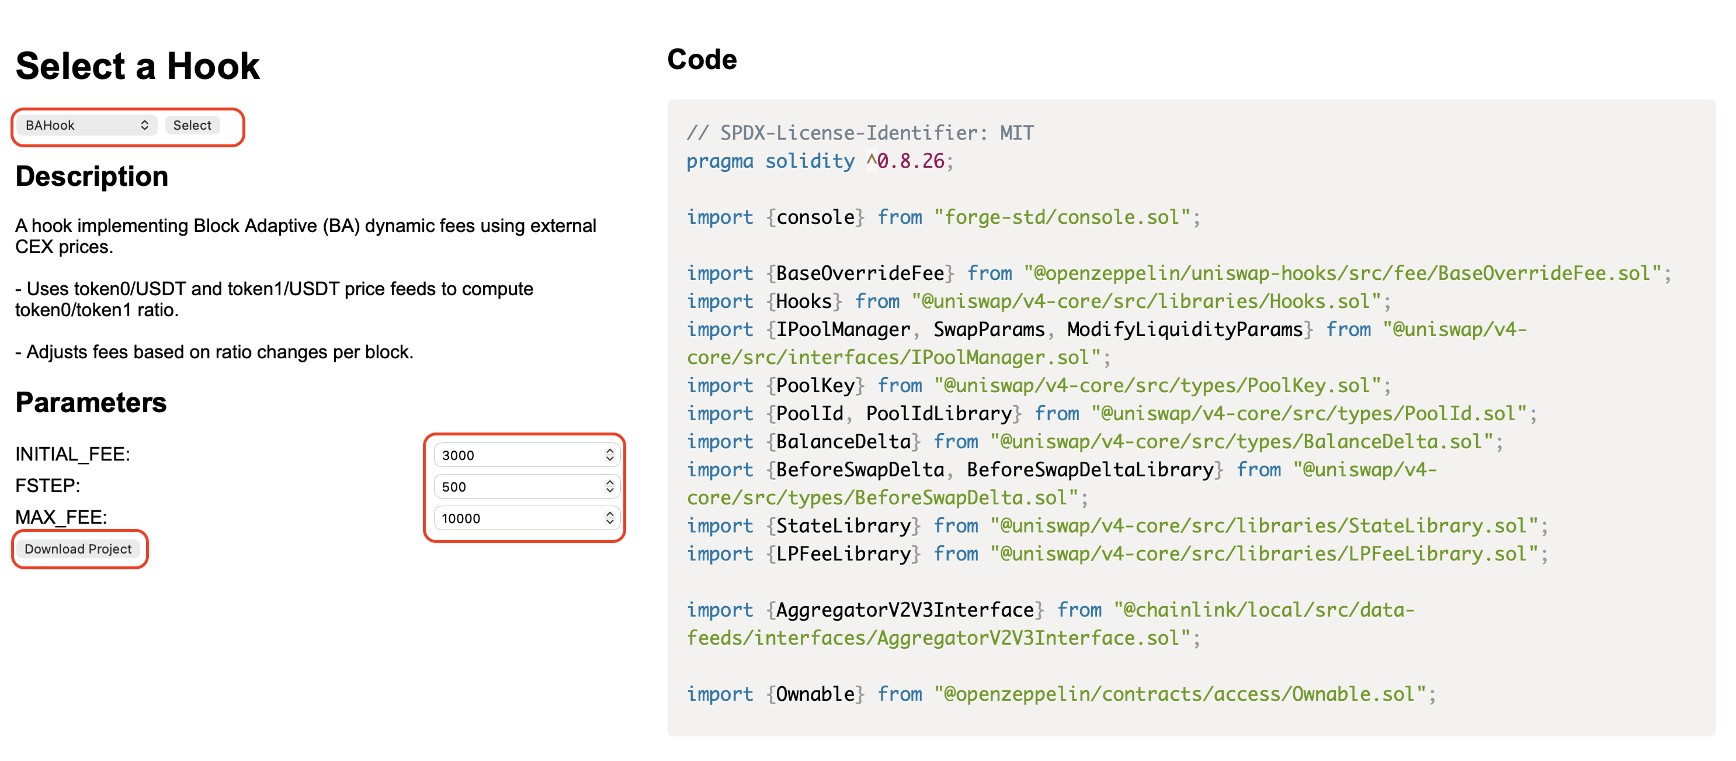
\includegraphics[width=\columnwidth]{Image/hook_configurator.png}
  \caption{Selecting a dynamic-fee template and its exposed parameters.}
  \label{fig:configurator}
\end{figure}

The code view updates with parameter changes (Fig.~\ref{fig:code}), allowing inspection before compilation. This transparency is important because fee units and bounds are protocol-specific: Uniswap v4 represents LP fees as \texttt{uint24} values in hundredths of a basis point~\cite{uniswapDynamicFees}. Compilation and tests remain necessary; the interface is not a security verifier.

The generated artifact preserves the user-selected numeric values but does not automatically establish semantic validity. For example, a minimum fee can be syntactically valid while exceeding a configured maximum, and an oracle-dependent hook can compile with feeds for the wrong assets. The intended validation pipeline therefore has three levels: schema checks at configuration time, Solidity compilation and unit tests after generation, and deployment-time checks for network addresses, hook permissions, and pool configuration. The prototype implements the generation and test workflow; stronger typed constraints are identified as future work rather than assumed here.

\begin{figure}[t]
  \centering
  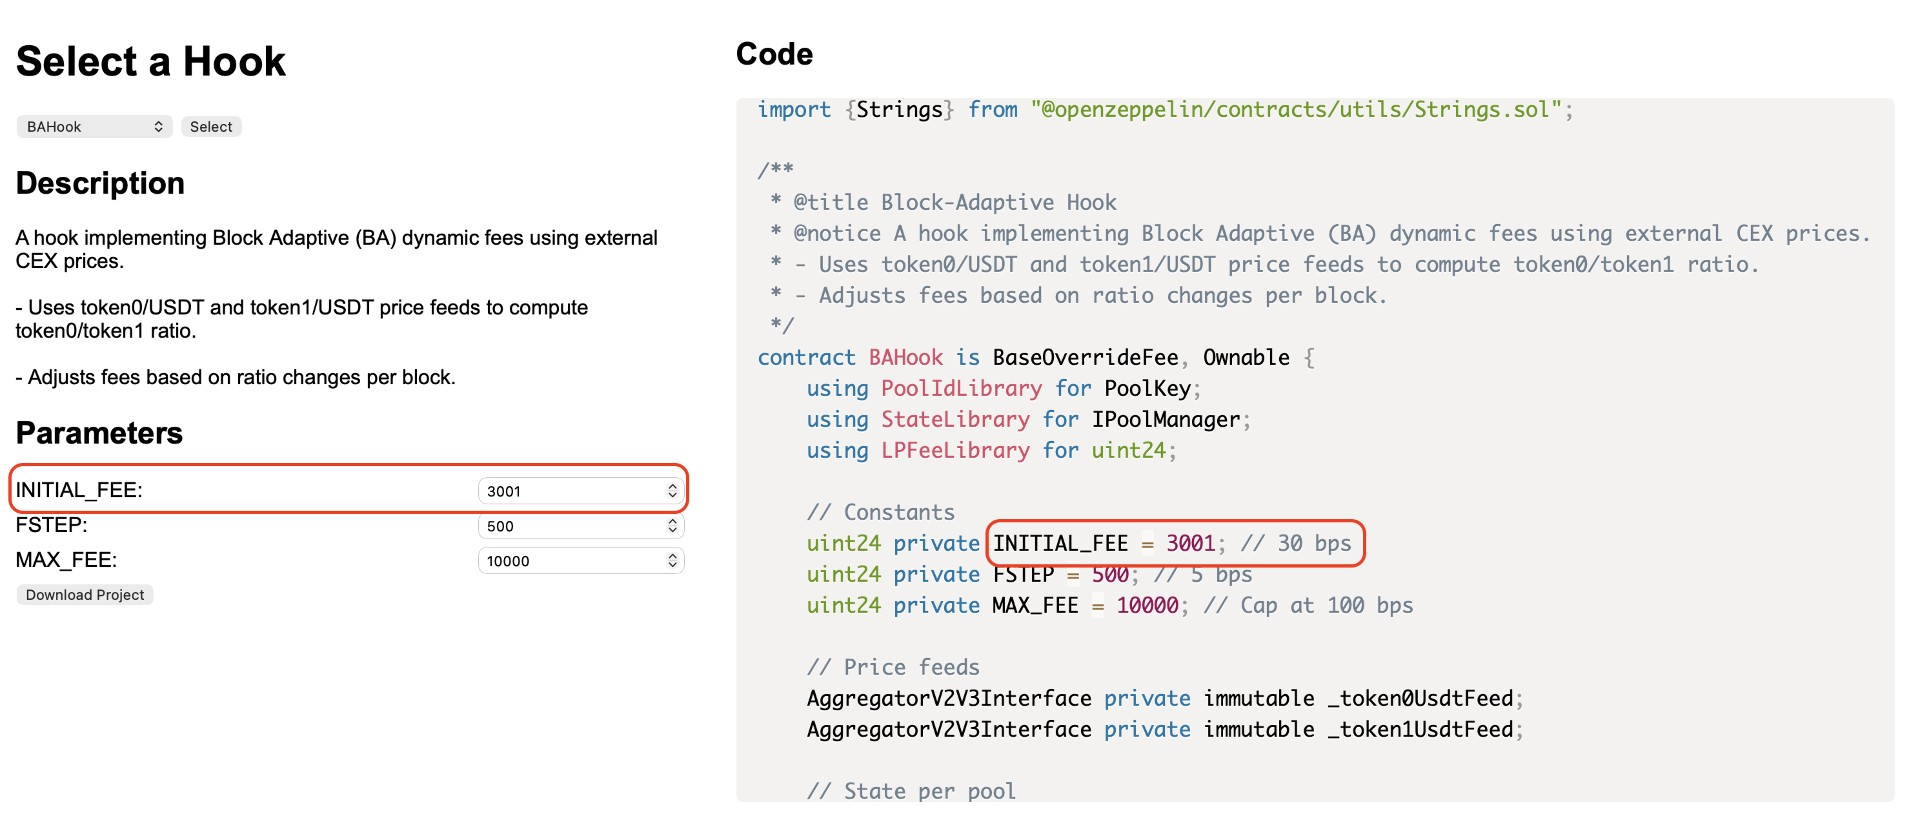
\includegraphics[width=\columnwidth]{Image/parameterized_code.png}
  \caption{Configured parameters reflected in the generated Solidity source.}
  \label{fig:code}
\end{figure}

\subsection{Hook Interface and Lifecycle}

The hook family reuses a fee-oriented base path consistent with OpenZeppelin's modular Uniswap hook design~\cite{openzeppelinHooks}. A representative block-adaptive implementation uses \texttt{poolManager()} to identify the authorized manager, \texttt{\_getPriceRatio()} to normalize two feeds and obtain their ratio, \texttt{\_afterInitialize()} to set initial state and directional fees, a fee selector for the swap direction, an owner-restricted setter where enabled, and \texttt{\_afterSwap()} to advance state after eligible swaps. Shared callback checks prevent arbitrary callers from invoking lifecycle entry points directly.

Let $r_b$ denote the external token-price ratio observed in block $b$:
\begin{equation}
  \Delta_b=\frac{r_b-r_{b-1}}{r_{b-1}}.
  \label{eq:blockchange}
\end{equation}
The policy maps the change, prior directional fees, and parameters to
\begin{equation}
  (f_b^{0\rightarrow1},f_b^{1\rightarrow0})=
  \mathcal{F}_{\mathrm{BA}}(\Delta_b,f_{b-1}^{0\rightarrow1},
  f_{b-1}^{1\rightarrow0};\theta),
  \label{eq:bapolicy}
\end{equation}
subject to $f_{\min}\le f_b^d\le f_{\max}$. Updating at most once per block avoids reacting repeatedly to a shared reference observation; deal-adaptive policies can instead update after individual swaps.

The library exposes specific policy templates, including a block-adaptive hook (\texttt{BAHook}) that adjusts fees based on external price ratio changes, a deal-adaptive hook (\texttt{DAHook}) for transaction-level updates, and volatility-based hooks utilizing Exponential Moving Average (EMA) and Welford’s online algorithm to react to trade volume variance.

Table~\ref{tab:hooks} summarizes the policies at the abstraction level supported by the available implementation report. The MEV-oriented template should be understood as applying specialized fee logic associated with the corresponding scenario; the artifact does not demonstrate complete detection or prevention of MEV. Likewise, the peg-stability template supplies peg-oriented behavior but is not evidence that a peg can be maintained under arbitrary liquidity or market shocks.

\begin{table*}[t]
  \caption{Dynamic-fee templates exposed by the framework.}
  \label{tab:hooks}
  \centering
  \footnotesize
  \begin{tabular}{p{2.2cm}p{3.2cm}p{4.4cm}p{5.2cm}}
    \toprule
    \textbf{Template} & \textbf{Update granularity} & \textbf{Primary signal or condition} & \textbf{Framework role}\\
    \midrule
    \texttt{BAHook} & At most once per block & Change in an external token-price ratio & Demonstrates block-adaptive directional fees\\
    \texttt{DAHook} & Individual trade & Deal-level state and swap characteristics & Demonstrates transaction-level adaptation\\
    \texttt{ABHook} & Block-level & External ratio with asymmetric response & Demonstrates distinct fees by swap direction\\
    MEV-charge hook & Policy-specific & Conditions encoded by the MEV-oriented rule & Provides a specialized charging template and tests\\
    Peg-stability hook & Policy-specific & Deviation from a target or peg-related state & Provides a template for peg-oriented fee behavior\\
    \bottomrule
  \end{tabular}
\end{table*}

The common per-swap path can be summarized as follows. First, the callback verifies the manager and resolves the swap direction. Second, the hook reads the policy state and, when required, normalized external observations. Third, it evaluates the policy and bounds the result. Fourth, it returns or stores the protocol-formatted fee. Finally, the post-swap callback updates only the state permitted by the policy's granularity. Separating selection from state advancement makes repeated execution within a block explicit and testable.

\subsection{Deployment and Export}

Hook permissions are derived from the deployed address. The deployment path must therefore mine a compatible \texttt{CREATE2} salt, or use Foundry test facilities to place code at a compatible address locally~\cite{uniswapHookDeployment}. The framework then deploys or resolves \texttt{PoolManager}, position management, and routing artifacts; creates mock tokens and price feeds; deploys the chosen hook; constructs the pool key; initializes price; and adds test liquidity. The expected permission bitmap is checked because a wrong salt can disable required callbacks or enlarge the hook's attack surface~\cite{uniswapSecurityFramework}.

The exported archive contains the configured hook, interfaces, scripts, tests, dependency declarations, remappings, historical-data utility, and instructions (Fig.~\ref{fig:project}). This is more reproducible than exporting a single contract, although complete experiment replication also requires pinned dependency revisions, compiler version, input data, initial pool state, and parameters.

For a replay to be independently identifiable, its manifest should include
\begin{equation}
  E=\langle C_{\theta},D,P_0,L_0,W,S\rangle,
  \label{eq:manifest}
\end{equation}
where $C_{\theta}$ is the configured contract, $D$ the dependency and compiler revisions, $P_0$ initial pool price, $L_0$ initial liquidity, $W$ the market-data window, and $S$ the swap-generation configuration. The current archive contains the executable project structure; recording all elements of $E$ is a concrete extension needed for artifact-level reproducibility.

\begin{figure}[t]
  \centering
  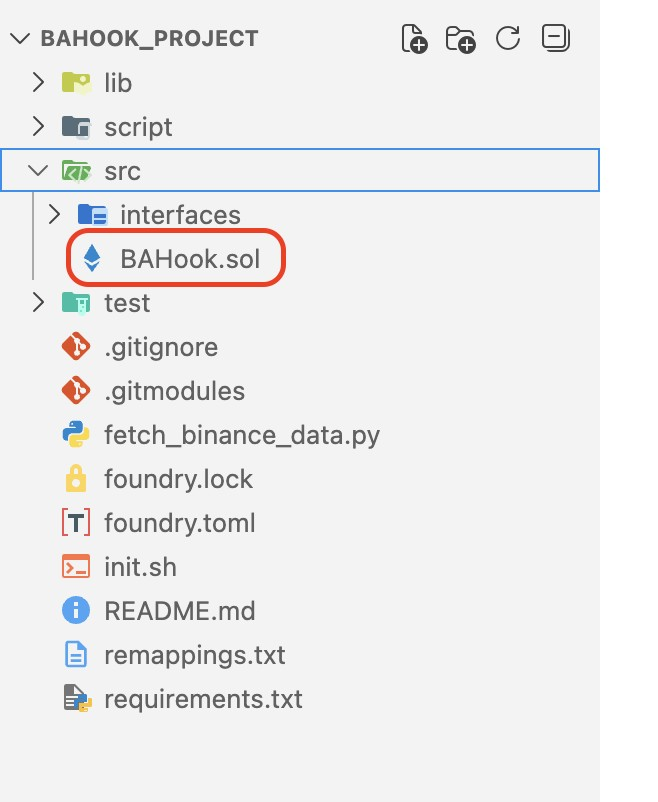
\includegraphics[width=.68\columnwidth]{Image/generated_project.png}
  \caption{Generated Foundry project for a configured hook.}
  \label{fig:project}
\end{figure}

To ensure strict reproducibility and auditability, the framework's off-chain layer utilizes a relational database (e.g., \texttt{PostgreSQL}) to maintain a complete history of parameter changes (\texttt{HookParamsHistory}), indexed blockchain events (\texttt{ChainEvent}), and pool state snapshots (\texttt{PoolStateSnapshot}). This allows any historical replay to be deterministically linked to the exact configuration and market state at the time of execution.

\subsection{Testing Strategy}

Testing is organized across three layers to ensure robustness. First, smart-contract tests (via Foundry) verify fee direction, bounds, update granularity, and edge values for each generated hook. Second, backend integration tests (in Go) validate the API layer, database state transitions, and historical data ingestion. Finally, end-to-end (e2e) tests (e.g., via Playwright) verify the complete user workflow, from web-based parameter configuration to project export and simulation execution. This multi-layer approach ensures that failures can be precisely localized to generation, deployment, contract execution, or data parsing.

% Testing is organized around the boundary between invariant framework behavior and variable policy behavior. Framework tests ask whether every generated hook can be deployed with the correct permissions, initialized through the same pool lifecycle, called only by the intended manager, and exercised by the common swap utilities. Policy tests ask whether a particular hook selects the expected direction, respects its bounds, and updates at the declared granularity. Separating these questions helps localize a failure: a deployment or callback failure belongs to shared infrastructure, whereas an unexpected fee with an otherwise valid swap belongs to the policy implementation.

The report identifies both common hook tests and specialized suites such as \texttt{MEVChargeHookFees.t.sol} and \texttt{PegStabilityHook.t.sol}. The simulation suite is distinct from unit tests. Unit tests cover fee direction, bounds, update granularity, and edge values. Deployment tests verify addresses, permissions, dependencies, and the pool key. Integration tests initialize liquidity and exercise callbacks through successful swaps, while replay tests validate observation ingestion, repeated execution, metrics, and plots. Adversarial cases should reject an unauthorized caller, stale feed, invalid parameter, and extreme input. Passing a replay is not a substitute for unit coverage because a long scenario may never reach these boundaries.

For a block-adaptive hook, a minimal transition suite should include $\Delta_b=0$, positive and negative changes, values that would cross both fee bounds, two swap directions, and multiple swaps assigned to the same block. It should verify that a same-block second swap does not advance block-level state unexpectedly. A deal-adaptive hook instead requires consecutive swaps to demonstrate that transaction-level updates occur. Oracle-informed tests should vary feed decimals, timestamps, sign, and the relative ordering of the two token prices. Owner-controlled setters need both authorized and unauthorized callers.

Generated projects also require differential checks against their templates. For a parameter vector $\theta$, the generated contract should differ only at declared substitution locations, compile under the recorded compiler, and retain the same callback permission set. A simple text comparison can identify accidental edits, while runtime tests confirm that the new constants affect the intended state. These checks are especially important because template generation occurs before deployment, after which an error may be immutable.

Finally, deterministic replay requires control over the chain and data context. Anvil fixes the local execution environment; the replay should additionally record block timestamps, observation order, token decimals, initial balances, liquidity, and any generated trade sizes. Without these fields, two executions can use the same nominal month and pair but produce different results. The manifest in Eq.~\eqref{eq:manifest} provides the core identifier, while an input checksum and event-level output would make exact comparison practical.

\section{Replay and Prototype Evaluation}
\label{sec:evaluation}

\subsection{Replay Procedure and Metrics}

The experiment form accepts a hook, year, month, and token pair. The backend obtains Binance kline observations~\cite{binanceKlines}, transforms them into the input consumed by \texttt{Simulation.t.sol}, and launches Forge. The test contract initializes mock tokens and a pool, acts as trader and LP, updates price-feed mocks, executes the swap sequence, and emits parseable output. The application extracts swap count, volume, directional fees, fee income, holdings, LP value, impermanent loss, and net loss, then generates the market and pool plots.

For swaps $i=1,\ldots,N$, let $q_i$ be the simulator's volume measure and $a_{i,j}^{f}$ the fee amount collected in token $j$. The direct aggregates are
\begin{equation}
  Q=\sum_{i=1}^{N}q_i, \qquad F_j=\sum_{i=1}^{N}a_{i,j}^{f}.
  \label{eq:aggregates}
\end{equation}
Token-denominated fees should remain separate unless a valuation price and time are declared. Once all values use a common numeraire, Eqs.~\eqref{eq:il}--\eqref{eq:netloss} provide the gross and fee-adjusted LP measures. The further conditions a conclusive comparison would require are set out in Sec.~\ref{sec:discussion}, and none is inferred from the prototype.

Historical CEX observations drive the offline scenario; Chainlink-compatible mocks provide the contract-readable interface. They are intentionally distinct roles. Replaying Binance data through a mock feed does not reproduce a live feed's source aggregation, heartbeat, deviation threshold, or latency.

\subsection{Prototype Execution}

The supplied execution contains 1,492 simulated swaps. Because the report does not identify a volume numeraire, no USD interpretation is assigned to the aggregate volume or token-denominated fee income.

To demonstrate that the framework correctly links market conditions to fee adjustments, Figure~\ref{fig:dynamic_fee_reaction} visualizes the core mechanism of the dynamic-fee hook in action over a representative window of 1,492 simulated swaps. The top panel shows the SHIB/ETH price ratio serving as the oracle input. The bottom panel shows the resulting dynamic fee parameter (in basis points). This two-panel view explicitly demonstrates the causal chain: as the price ratio exhibits higher variance, the hook scales the fee upward from the base rate, directly reflecting the calculated market volatility while respecting the configured bounds. This confirms that the integration path functions as designed, even though this single trace does not constitute a full economic baseline comparison.

\begin{figure*}[t]
  \centering
  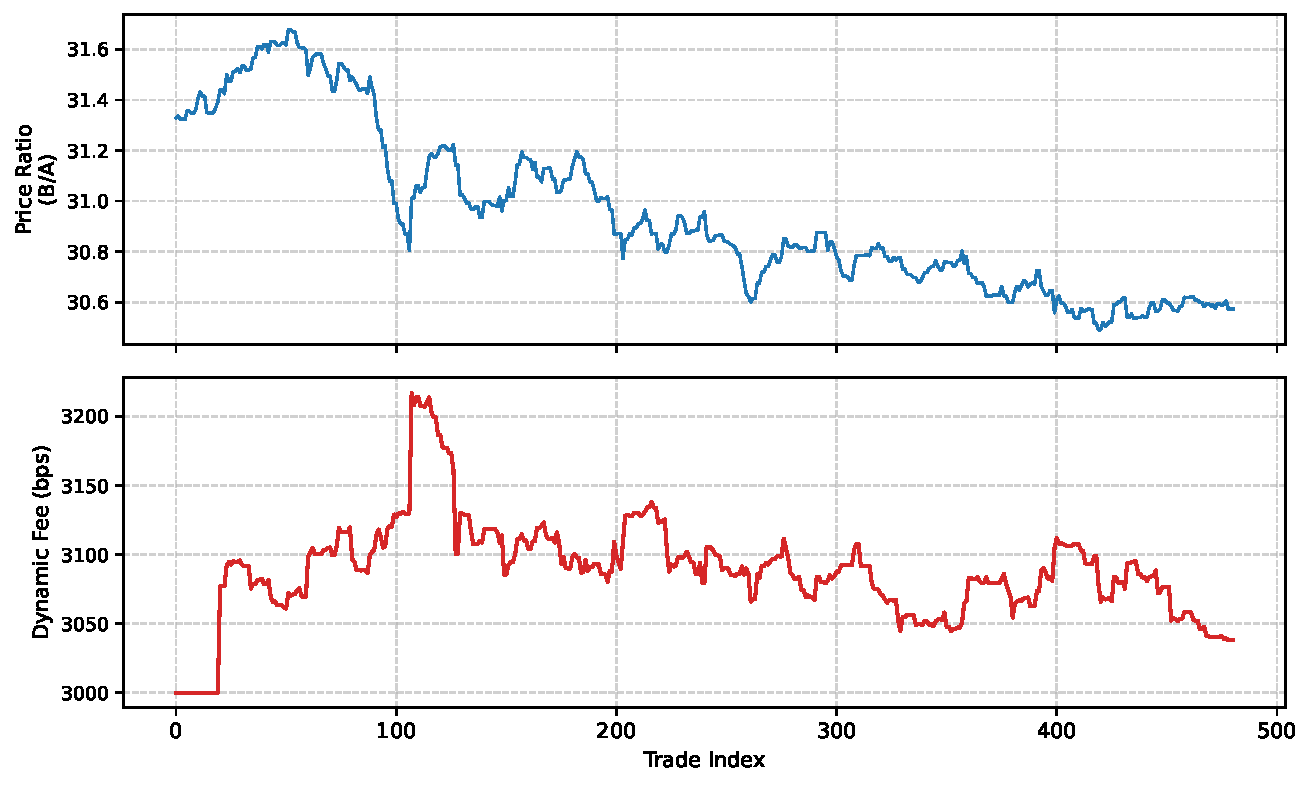
\includegraphics[width=0.8\linewidth]{Image/dynamic_fee_reaction.pdf}
  \caption{Core mechanism of the dynamic-fee hook in action. \textbf{(Top)} Price ratio (SHIB/ETH) showing market movement. \textbf{(Bottom)} The resulting dynamic fee parameter (in basis points), demonstrating how the policy scales the fee in response to underlying market volatility.}
  \label{fig:dynamic_fee_reaction}
\end{figure*}

The execution verifies the integration path: configure a hook, deploy local contracts, inject observations, execute swaps, collect contract output, and render results. It does not establish economic superiority. The artifact provides no same-trace fixed-fee baseline, repeated trials, uncertainty intervals, gas measurements, or complete specification of trade sizing and data cleaning. Accordingly, the paper claims feasibility rather than reduced LP loss.

\section{Security, Validity, and Discussion}
\label{sec:discussion}

\subsection{Security Considerations}

Dynamic-fee hooks execute inside the swap lifecycle and enlarge the trusted code surface. Production implementations should restrict setters, accept callbacks only from the designated \texttt{PoolManager}, enforce protocol and policy fee bounds, normalize oracle decimals, reject stale or nonpositive rounds, and handle division and casts safely. Address-permission validation is essential. Uniswap's security guidance emphasizes that incorrectly encoded permissions or custom deltas can produce unintended execution paths~\cite{uniswapSecurityFramework}.

The web layer crosses a separate trust boundary. Hook names should be allowlisted; parameter types and ranges should be validated before substitution; generated files should be written to isolated temporary locations; and simulator arguments must not become shell fragments. Resource limits are needed because compilation and replay are user-triggered operations. Exported projects should pin revisions to prevent later dependency changes from silently altering a result.

Between the contract and application layers sits a data boundary: the implementation must check feed identity, sign, decimals, and timestamp, and define behavior for unavailable observations. Contract- and data-boundary threats admit code-level tests; application-layer risks and historical-replay bias instead require common baselines, multiple regimes, and explicit experimental reporting.

\subsection{Validity and Design Trade-offs}

Local execution provides deterministic debugging but not public-chain market microstructure. Historical replay omits mempool visibility, block-builder ordering, latency, gas competition, strategic arbitrage, and endogenous routing. Results also depend on initial price and liquidity, token decimals, observation frequency, trade sizes, valuation time, and the share of informed flow. One pair and interval cannot establish generality, particularly across volatile, stablecoin, and shallow-liquidity markets.

The framework's main benefit is separation of concerns: researchers can change $\mathcal{F}$ in Eq.~\eqref{eq:policy} while retaining deployment, ingestion, and analysis. Generated source remains inspectable, and mocks make integration tests repeatable. The trade-off is that textual template substitution is less safe and expressive than a typed policy language; mock feeds validate calls but not production oracle behavior; and console parsing is less robust than a structured event-level result format.

Developing robust backtesting infrastructure for AMM strategies is an active area of research~\cite{urusov2025backtesting}. A controlled economic study within such a framework should hold the trace, initial reserves, liquidity range, valuation convention, and random seed constant while varying only the policy. It should compare all hooks with static-fee baselines and report LP value, fee income, IL or LVR, net outcome, retained volume, mean and distribution of fees, gas overhead, and runtime. Multiple pairs, volatility regimes, and repeated windows are required for uncertainty estimates. These additions are future evaluation work, not evidence inferred from the current trace.

The next implementation steps are therefore a typed parameter schema, containerized and version-pinned experiments, event-level result export, property-based tests for fee bounds and callback authorization, stale-oracle fault injection, and testnet validation. Together they would turn the current development framework into a stronger comparative research testbed. Furthermore, the framework is designed to easily accommodate emerging fee paradigms, such as trade-size-aware Impermanent-Loss Trimming (ILT) mechanisms and path-independent fee structures that preserve composability guarantees under transaction fragmentation \cite{11575501}.

\section{Conclusion}

This paper presented an end-to-end framework for configuring, deploying, and replay-testing dynamic-fee hooks on Uniswap v4. Shared contracts and scripts isolate policy logic from protocol bootstrap; the web interface exposes parameters and source; and the experiment path connects historical observations to local execution and metrics. A 1,492-swap ETH/SHIB trace demonstrates that the integrated workflow operates. It does not prove that a dynamic policy outperforms static fees. The contribution is transparent, reusable infrastructure that enables such policies to be implemented and, with controlled baselines and broader traces, compared reproducibly.

\IfFileExists{IEEEtran.bst}{\bibliographystyle{IEEEtran}}{\bibliographystyle{unsrt}}
\bibliography{reference}
\end{document}
